\documentclass{beamer}
\usepackage{hyperref}
\hypersetup{colorlinks=true,}
\usepackage{url}
\usepackage{svg}
\usepackage{multicol}
\usepackage{smartdiagram}
\smartdiagramset{font=\sffamily,text width = 5cm, back arrow disabled}
\usepackage{listings}
\usepackage{xcolor}
\usepackage{menukeys}
\usepackage[backend=biber, style=apa]{biblatex}
\addbibresource{references/tosref_v8.bib}

\lstdefinelanguage{HolyC}{ morekeywords={F64, U64, I64, U32, I32, U16, I16, I8, U8, Bool, U0, if, for, switch, case, break}, sensitive=false, morecomment=[l]{//}, morecomment=[s]{/*}{*/}, morestring=[b]", alsoletter={.}, }

\usetheme{Ilmenau}
\usecolortheme{default}
\useoutertheme{miniframes}

\setbeamertemplate{headline}{
	\begin{beamercolorbox}[wd=\paperwidth,ht=8ex,dp=1.125ex]{section in head/foot} \vfill \insertnavigation{1.02\paperwidth} \vfill\end{beamercolorbox}
}

\title{TempleOS and HolyC}
\author{Bc. Eduard Jurášek}
\institute{ FIS VŠE, Prague }
\date{\today}

\begin{document}
	\begin{frame}
		\titlepage

		\begin{figure}
			\centering
			
\includegraphics[width=0.2\linewidth]{images/publicdomain.png}
		\end{figure}
		All content related to Terry A. Davis, TempleOS, J Operating System,
		SparrowOS, or LoseThos should be considered public domain.
	\end{frame}

	\begin{frame}
		\frametitle{Table of Contents}
		\begin{multicols}{3}
			\tableofcontents
		\end{multicols}
	\end{frame}

	\section{Notes}
	\begin{frame}
		\frametitle{Academic work}
		This work was written as a seminar project for a 4IZ552 Course - Electronic Typesetting
		and Publishing at Faculty of Informatics and Statistics at Prague University
		of Economics and Business.
		\begin{figure}
			\centering
			
\includegraphics[width=0.5\linewidth]{images/FIS_1_logo_cmyk.eps}
		\end{figure}
		Feel free to find out more at \url{https://fis.vse.cz/} faculty website.
	\end{frame}
	\begin{frame}
		\frametitle{Important remarks}
		The author of this presentation prepared the slides with respect to Terry A.
		Davis, who was affected with his mental illness, and primarily focuses on
		the technical aspect of the TempleOS and HolyC.

		Additionally, the author describes the problems of Terry as they are, in a
		way not to harm or make fun of him.

		If you find something inappropriate in this presentation, let me know at \href{mailto:jure01@vse.cz}{jure01@vse.cz}
		email address.

		Thank you.
	\end{frame}

	\section[Intro]{Introduction}
	\begin{frame}
		\frametitle{Quotes}
		\begin{quote}
			Davis was clearly a gifted programmer – writing an entire operating system
			is no small feat – and it was sad to see him affected by his mental illness.

			\flushright -- Thom Holwerda
		\end{quote}

		\vspace{1em}
		\begin{quote}
			You can imagine how over time one man might build a house, but this is
			like building a skyscraper, on your own! \flushright -- Anonymous
		\end{quote}
	\end{frame}

	\section[T. Davis]{Terry Davis}
	\subsection{Basic information}
	\begin{frame}
		\frametitle{About Terry A. Davis}
		\begin{columns}
			\begin{column}{0.6\textwidth}
				\begin{itemize}
					\item Dec. 15, 1969 – Aug. 11, 2018

					\item Electrical engineer and programmer

					\item TicketMaster employee (1990 – 1996)

					\item Diagnosed with bipolar disorder and schizophrenia

					\item Deeply believed in God
				\end{itemize}
			\end{column}
			\begin{column}{0.25\textwidth}
				\begin{figure}
					\centering
					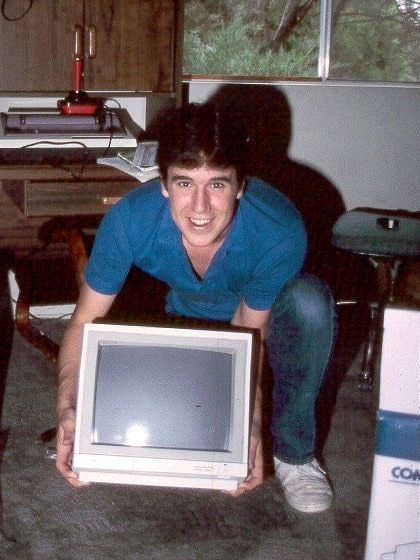
\includegraphics[width=\linewidth]{images/terry_1.jpg}
					\caption{Young Terry Davis}
					\label{fig:terry-young}
				\end{figure}
			\end{column}
		\end{columns}
		Image by \cite{davis_terry_2017}.
	\end{frame}

	\subsection{Development Era}
	\begin{frame}
		\frametitle{Development Era}
		\begin{itemize}
			\item Started development after God told him

			\item Shared his work on Reddit, OSdev, hackernews

			\item Used losethos and TrivialSollutions usernames

			\item Got banned frequently

			\item Many posts deleted for rudeness and spam

			\item Uploaded TempleOS videos on YouTube later

			\item Gained community of supporters and trolls
		\end{itemize}
	\end{frame}

	\subsection{Homeless Era}
	\begin{frame}
		\frametitle{Homeless Era}
		\begin{columns}
			\begin{column}{0.7\textwidth}
				\begin{itemize}
					\item Denied medication to increase creativity

					\item Sentenced for attacking his father

					\item Lived in a van as homeless

					\item Deleted most videos from his YouTube

					\item Died after being hit by a train
				\end{itemize}
			\end{column}
			\begin{column}{0.3\textwidth}
				\begin{figure}
					\centering
					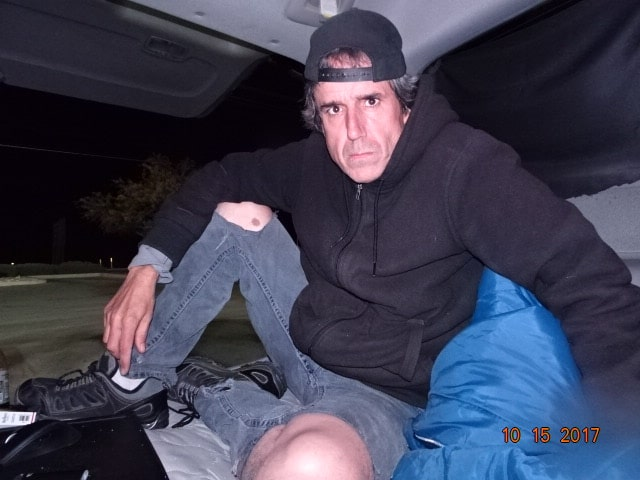
\includegraphics[width=\linewidth]{images/terry_2.jpg}
					\caption{Terry in a van}
					\label{fig:terry-van}
				\end{figure}
			\end{column}
		\end{columns}
		Image by \cite{davis_terry_2017}.
	\end{frame}

	\subsection{Controversies}
	\begin{frame}
		\frametitle{Controversies}
		\begin{itemize}
			\item Use of profane and offensive language

			\item Racist and homophobic slurs

			\item Paranoid about CIA "Glowies"

			\item Delusional relationship with Diana

			\item Narcissist traits

			\item Flame wars on forums and his website
		\end{itemize}

		\vspace{1em}
		\frametitle{Quotes}
		\begin{quote}
			I'm the smartest programmer that ever lived. \flushright -- Terry A. Davis
		\end{quote}
	\end{frame}

	\section[TOS]{TempleOS}
	\subsection{Ancestors}
	\begin{frame}
		\frametitle{Ancestors}

		\begin{columns}
			\begin{column}{0.33\textwidth}
				\scalebox{0.6}{ \smartdiagram[flow diagram]{Doors, Davos, J Operating System, LoseThos!, SparrowOS, TempleOS}
				}
			\end{column}

			\begin{column}{0.33\textwidth}
				\begin{figure}
					\centering
					
\includegraphics[width=1.0\linewidth]{images/losethos.png}
					\caption{LoseThos! logo}
					\label{fig:losethos}
				\end{figure}
				Image by \cite{terry_a_davis_taught_us_how_to_talk_to_god__davisanism_losethos_2023}
			\end{column}

			\begin{column}{0.33\textwidth}
				\begin{figure}
					\centering
					
\includegraphics[width=0.5\linewidth]{images/sparrow.png}
					\caption{SparrowOS logo}
					\label{fig:sparrowos}
				\end{figure}
				Image by \cite{absolute_terry_davis_32_2021}.
			\end{column}
		\end{columns}
	\end{frame}

	\begin{frame}
		\frametitle{What is TempleOS?}
		\begin{columns}
			\begin{column}{0.5\textwidth}
				\begin{itemize}
					\item 64-bit operating system

					\item Created by Terry A. Davis

					\item God's Third Temple

					\item About 100 000 lines of code

					\item Developed over 10 years soley by Terry
				\end{itemize}
			\end{column}

			\begin{column}{0.5\textwidth}
				\begin{figure}
					\centering
					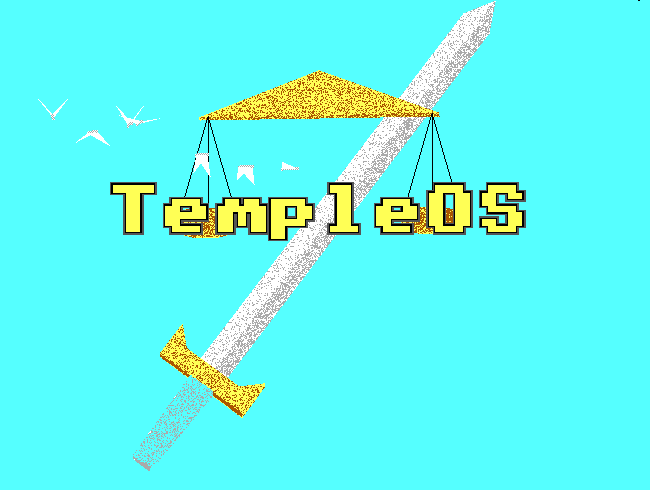
\includegraphics[width=0.5\linewidth]{images/TempleOS_logo.png}
					\caption{TempleOS logo}
					\label{fig:tos_logo}
				\end{figure}
				\centering
				Image by \cite{davis_terry_2017}.
			\end{column}
		\end{columns}
	\end{frame}

	\begin{frame}
		\frametitle{What makes TempleOS unique?}
		\begin{columns}
			\begin{column}{0.5\textwidth} % Specify the width of the column
				\begin{itemize}
					\item Ring 0 - everything runs in kernel

					\item Very own RedSea file system

					\item HolyC language

					\item Encoding of files

					\item Own 2D and 3D libraries

					\item Design
				\end{itemize}
			\end{column}

			\begin{column}{0.5\textwidth} % Specify the width of the column
				\begin{itemize}
					\item Backstory

					\item 16-bit colors

					\item 640$\times$480 resolution

					\item Single Vice Audio
				\end{itemize}
			\end{column}
		\end{columns}
	\end{frame}

	\begin{frame}
		\frametitle{How can I download TempleOS?}
		\begin{itemize}
			\item Official website \url{https://templeos.org/}

			\item The size of ISO is 15.6 MB!

			\item Or try it online, eg. at \url{https://instantworkstation.com/virtual-machine}
		\end{itemize}
	\end{frame}

	\begin{frame}
		\frametitle{System requirements}
		\begin{itemize}
			\item 512 MB of RAM

			\item 64-bit, x86 processors

			\item Keyboard

			\item Runs in virtual machines too
		\end{itemize}
	\end{frame}

	\begin{frame}
		\frametitle{Keyboard shortcuts}
		\begin{itemize}
			\item \keys{Space} $\rightarrow$ Left Click

			\item \keys{Enter} $\rightarrow$ Right Click

			\item \keys{F1} $\rightarrow$ Help

			\item \keys{Ctrl + M} $\rightarrow$ Personal Menu

			\item \keys{Ecs} $\rightarrow$ Save and exit

			\item \keys{Shift + Ecs} $\rightarrow$ Abort and exit

			\item \keys{Windows (Super)} $\rightarrow$ Pull-Down Menu
		\end{itemize}
	\end{frame}

	\section{GodWorks}
	\begin{frame}
		\frametitle{Keyboard shortcuts}
		\begin{itemize}
			\item \keys{F7} $\rightarrow$ God Word

			\item \keys{Shift + F7} $\rightarrow$ God Passage

			\item \keys{F6} $\rightarrow$ God Song

			\item \keys{Shift + F6} $\rightarrow$ God Doodle

			\item \keys{Ctrl + Alt + B} $\rightarrow$ Bible
		\end{itemize}

		\vspace{1em}

		\frametitle{Quotes}
		\begin{quote}
			I like elephants and God likes elephants... If you don't wanna go for
			realism, you can go for better than realism... How about an elephant with
			blue eyes! \flushright -- Terry A. Davis
		\end{quote}
	\end{frame}

	\begin{frame}
		\frametitle{God Word}
		Generates random words
		\begin{figure}
			\centering
			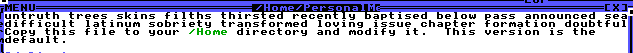
\includegraphics[width=0.95\linewidth]{images/god_word.png}
			\caption{God Word. Own work.}
			\label{fig:god_work}
		\end{figure}
	\end{frame}

	\begin{frame}
		\frametitle{God Passage}
		Opens random passage from Bible
		\begin{figure}
			\centering
			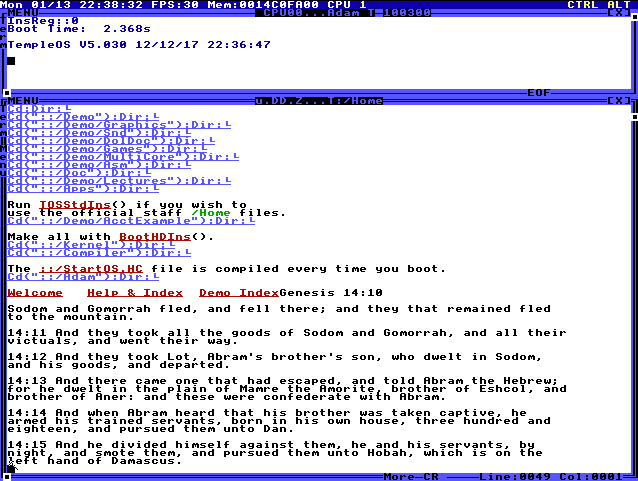
\includegraphics[width=0.6\linewidth]{images/god_passage.png}
			\caption{God Passage. Own work.}
			\label{fig:god_passage}
		\end{figure}
	\end{frame}

	\begin{frame}
		\frametitle{God Song}
		Generates random songs
		\begin{figure}
			\centering
			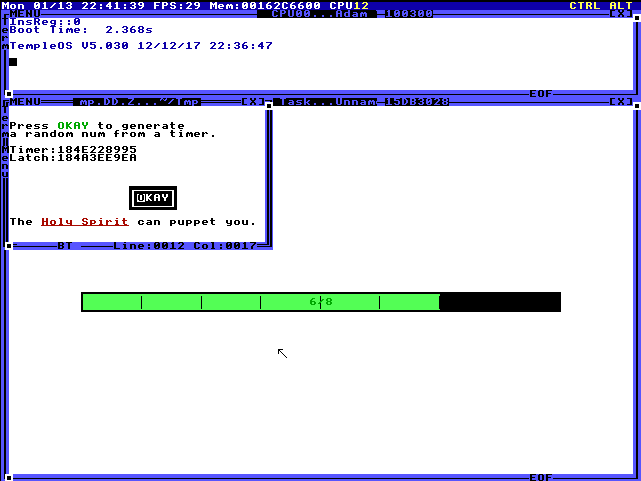
\includegraphics[width=0.6\linewidth]{images/god_song.png}
			\caption{God Song. Own work.}
			\label{fig:gods_song}
		\end{figure}
	\end{frame}

	\begin{frame}
		\frametitle{Risen - TempleOS Hymn}

		Original available here: \url{https://www.youtube.com/watch?v=hmjU-6tkEc8}

		\vspace{1em}

		Community Remixes:
		\begin{itemize}
			\item Remix

				\url{https://www.youtube.com/watch?v=IdYMA6hY_74}

			\item Techno

				\url{https://www.youtube.com/watch?v=mR8Cg1DnoRU}

			\item Synthwave

				\url{https://www.youtube.com/watch?v=liMUF306cHs}
		\end{itemize}
	\end{frame}

	\begin{frame}
		\frametitle{God Doodle}
		Draws random doodle
		\begin{figure}
			\centering
			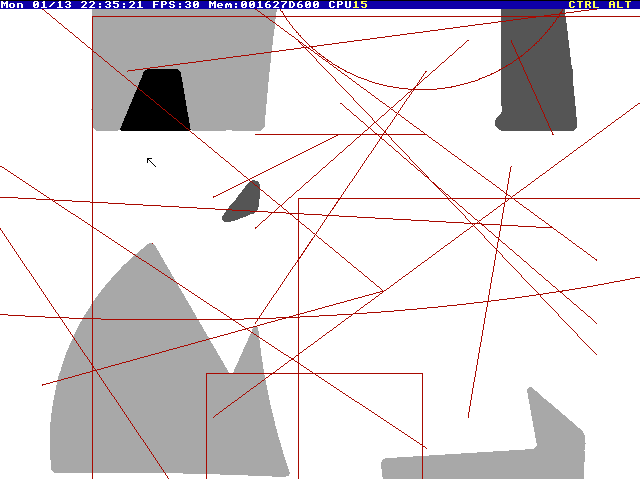
\includegraphics[width=0.6\linewidth]{images/god_doodle.png}
			\caption{God Doodle. Own work.}
			\label{fig:gods_doodle}
		\end{figure}
	\end{frame}

	\begin{frame}
		\frametitle{Bible}
		Bible implemented directly to TempleOS
		\begin{figure}
			\centering
			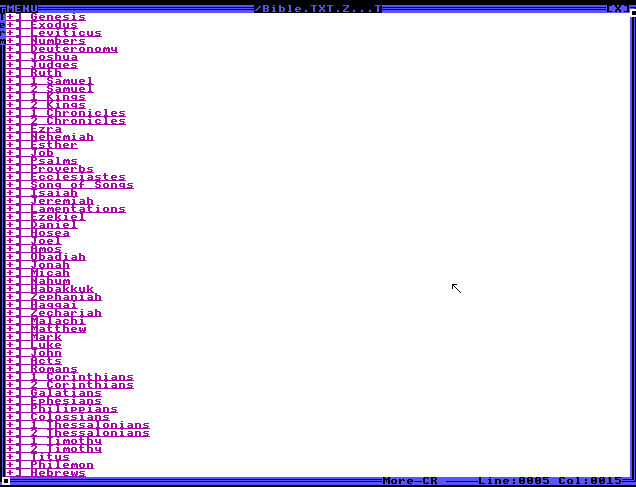
\includegraphics[width=0.6\linewidth]{images/bible.png}
			\caption{Bible. Own work.}
			\label{fig:bible}
		\end{figure}
	\end{frame}

	\section[TOS Menu]{TempleOS Menu}
	\subsection{Fun Games}
	\begin{frame}
		\frametitle{Fun Games Menu}
		\begin{figure}
			\centering
			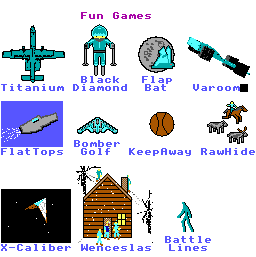
\includegraphics[width=0.6\linewidth]{images/fun_games.png}
			\caption{Fun games menu. Own work.}
			\label{fig:fun_games}
		\end{figure}
	\end{frame}

	\begin{frame}
		\frametitle{Titanium}
		Defender game
		\begin{figure}
			\centering
			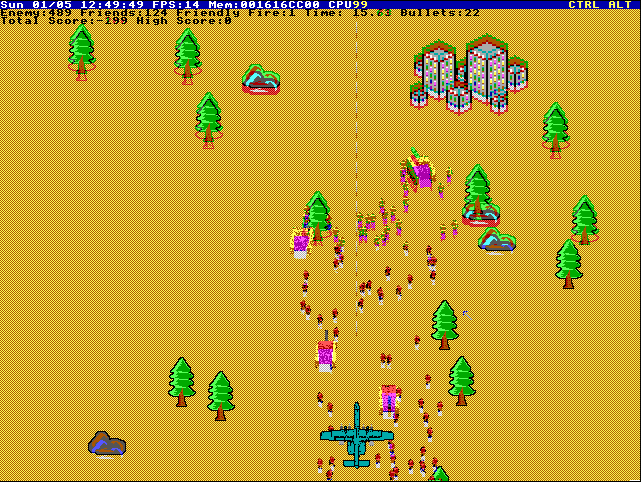
\includegraphics[width=0.6\linewidth]{images/titanium.png}
			\caption{Titanium. Own work.}
			\label{fig:titanium}
		\end{figure}
	\end{frame}

	\begin{frame}
		\frametitle{Black Diamond}
		Slope skiing game
		\begin{figure}
			\centering
			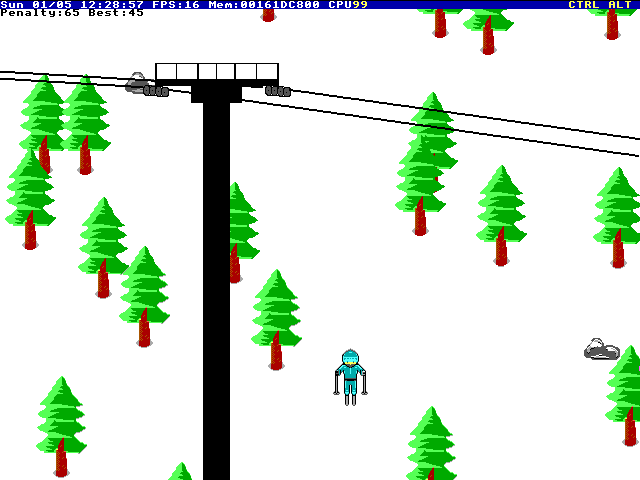
\includegraphics[width=0.6\linewidth]{images/black_diamond.png}
			\caption{Black Diamond. Own work.}
			\label{fig:black_diamond}
		\end{figure}
	\end{frame}

	\begin{frame}
		\frametitle{Flapbat}
		Bat eating bugs game
		\begin{figure}
			\centering
			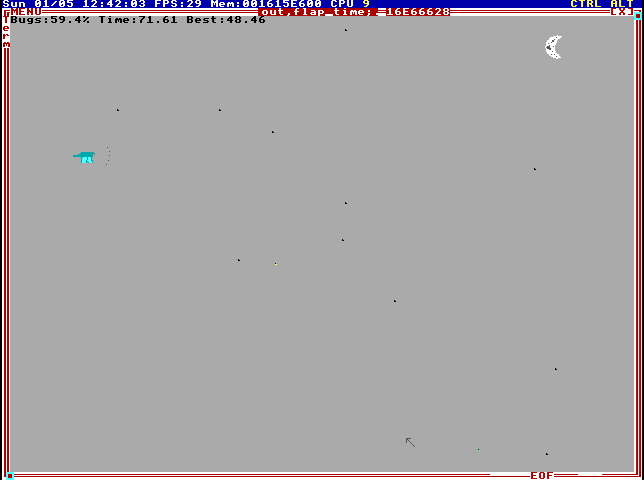
\includegraphics[width=0.6\linewidth]{images/flapbat.png}
			\caption{Flapbat. Own work.}
			\label{fig:flapbat}
		\end{figure}
	\end{frame}

	\begin{frame}
		\frametitle{Varoom}
		Cart racing simulator
		\begin{figure}
			\centering
			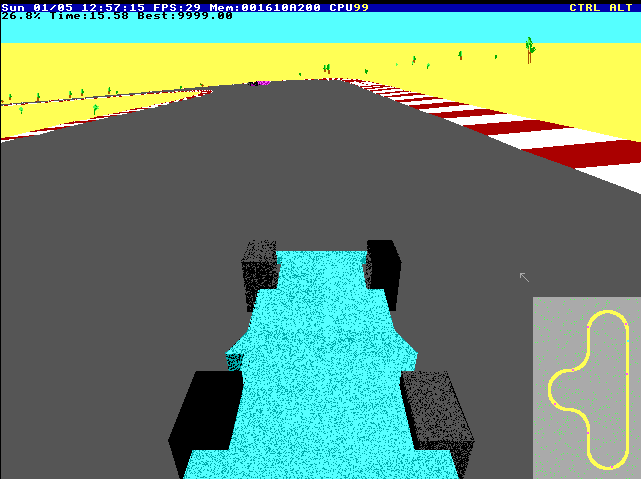
\includegraphics[width=0.6\linewidth]{images/varoom.png}
			\caption{Varrom. Own work.}
			\label{fig:varoom}
		\end{figure}
	\end{frame}

	\begin{frame}
		\frametitle{FlatTops}
		Battleship game
		\begin{figure}
			\centering
			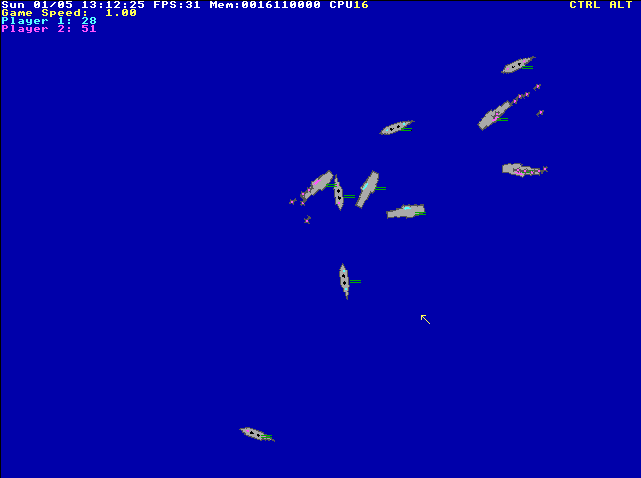
\includegraphics[width=0.6\linewidth]{images/flat_tops.png}
			\caption{FlatTops. Own work.}
			\label{fig:flat_tops}
		\end{figure}
	\end{frame}

	\begin{frame}
		\frametitle{BomberGolf}
		Bomber plane game
		\begin{figure}
			\centering
			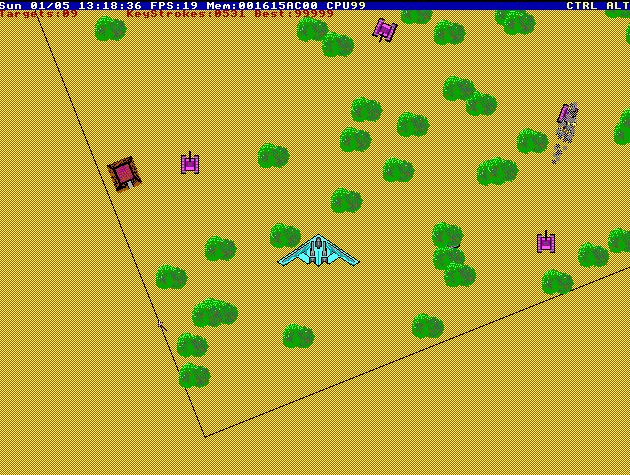
\includegraphics[width=0.6\linewidth]{images/bomber_golf.png}
			\caption{BomberGolf. Own work.}
			\label{fig:bomber_golf}
		\end{figure}
	\end{frame}

	\begin{frame}
		\frametitle{KeepAway}
		Basketball game
		\begin{figure}
			\centering
			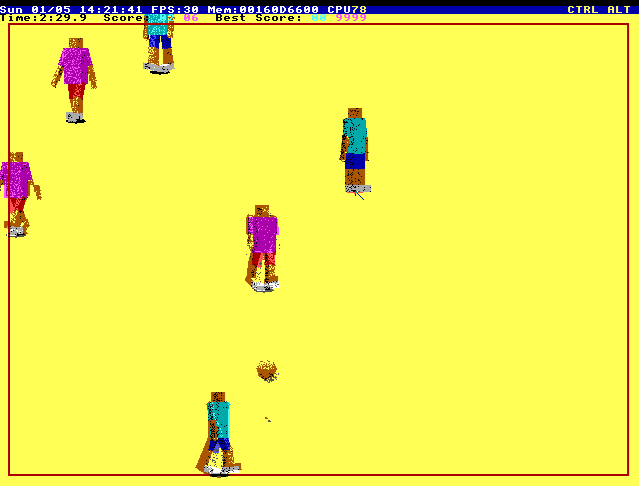
\includegraphics[width=0.6\linewidth]{images/keep_away.png}
			\caption{KeepAway. Own work.}
			\label{fig:keep_away}
		\end{figure}
	\end{frame}

	\begin{frame}
		\frametitle{Rawhide}
		Game where the goal is to round up the cattle
		\begin{figure}
			\centering
			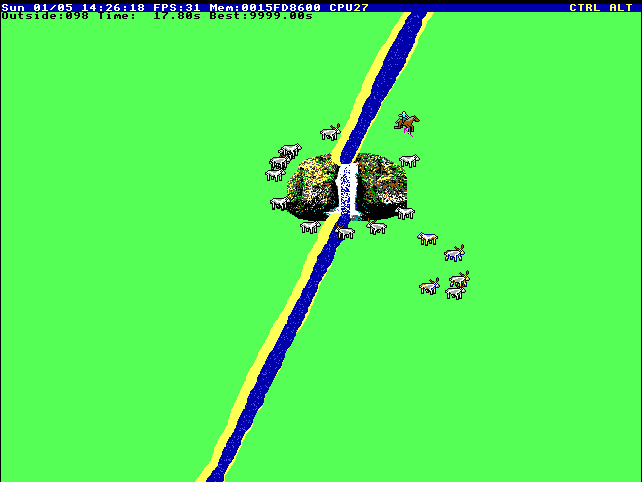
\includegraphics[width=0.6\linewidth]{images/rawhide.png}
			\caption{Rawhide. Own work.}
			\label{fig:rawhide}
		\end{figure}
	\end{frame}

	\begin{frame}
		\frametitle{X-Caliber}
		Spaceship shooting plasma balls game
		\begin{figure}
			\centering
			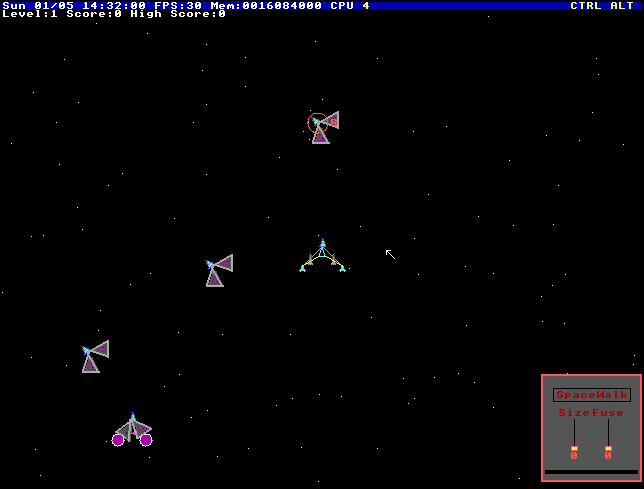
\includegraphics[width=0.6\linewidth]{images/xcaliber.png}
			\caption{X-Caliber. Own work.}
			\label{fig:xcaliber}
		\end{figure}
	\end{frame}

	\begin{frame}
		\frametitle{Wenceslas}
		Game where the goal is to guide peasants to warm
		\begin{figure}
			\centering
			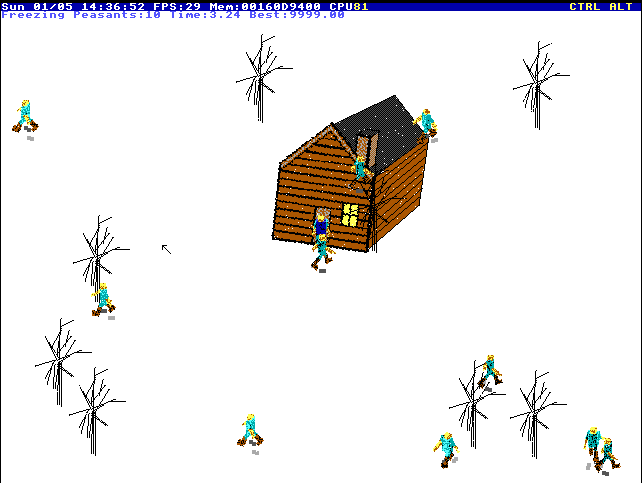
\includegraphics[width=0.6\linewidth]{images/wenceslas.png}
			\caption{Wenceslas. Own work.}
			\label{fig:wenceslas}
		\end{figure}
	\end{frame}

	\begin{frame}
		\frametitle{Battlelines}
		Two battle lines eliminating each other game
		\begin{figure}
			\centering
			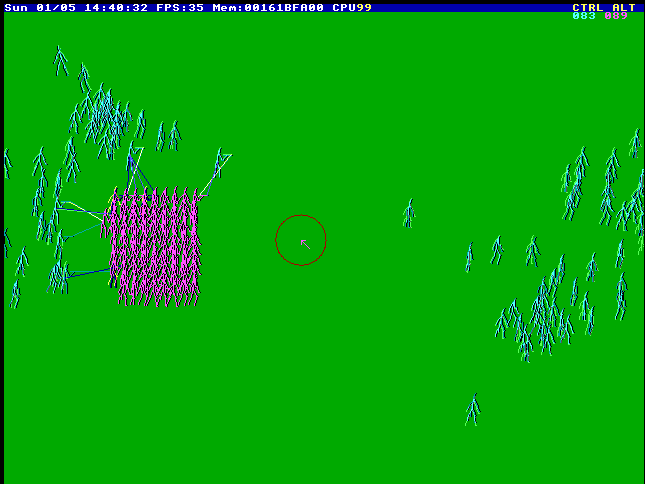
\includegraphics[width=0.6\linewidth]{images/battle_lines.png}
			\caption{Battlelines. Own work.}
			\label{fig:ebattle_lines}
		\end{figure}
	\end{frame}

	\subsection{Unfun Games}
	\begin{frame}
		\frametitle{Unfun Games}
		\begin{figure}
			\centering
			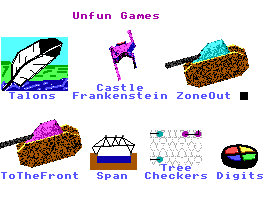
\includegraphics[width=0.5\linewidth]{images/unfun_games.png}
			\caption{Unfun Games. Own work.}
			\label{fig:unfun_games}
		\end{figure}
		\vspace{0.5em}

		\frametitle{Quotes}
		\begin{quote}
			Write games,don't play them. \flushright -- Terry A. Davis
		\end{quote}
	\end{frame}

	\begin{frame}
		\frametitle{Talons}
		Bird catching fish simulator
		\begin{figure}
			\centering
			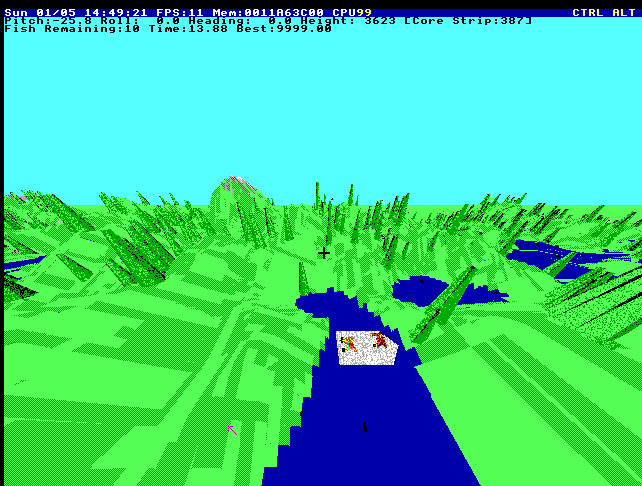
\includegraphics[width=0.6\linewidth]{images/talons.png}
			\caption{Talons. Own work.}
			\label{fig:talons}
		\end{figure}
	\end{frame}

	\begin{frame}
		\frametitle{Castle Frankentein}
		DOOM-like game
		\begin{figure}
			\centering
			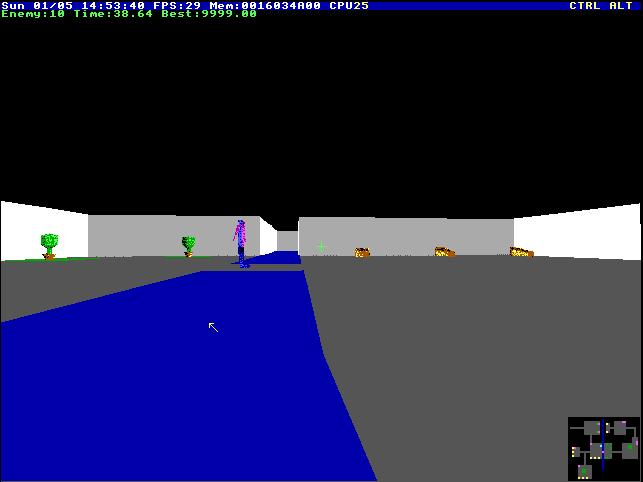
\includegraphics[width=0.6\linewidth]{images/castle_frankenstein.png}
			\caption{Castle Frankenstein. Own work.}
			\label{fig:castle_frankenstein}
		\end{figure}
	\end{frame}

	\begin{frame}
		\frametitle{Zone Out}
		Tank paintball game
		\begin{figure}
			\centering
			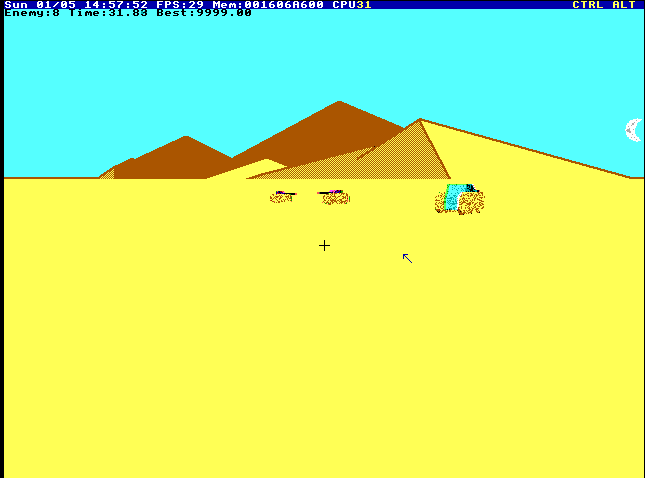
\includegraphics[width=0.6\linewidth]{images/zone_out.png}
			\caption{Zone Out. Own work.}
			\label{fig:zone_out}
		\end{figure}
	\end{frame}

	\begin{frame}
		\frametitle{To The Front}
		Militant king war strategy game
		\begin{figure}
			\centering
			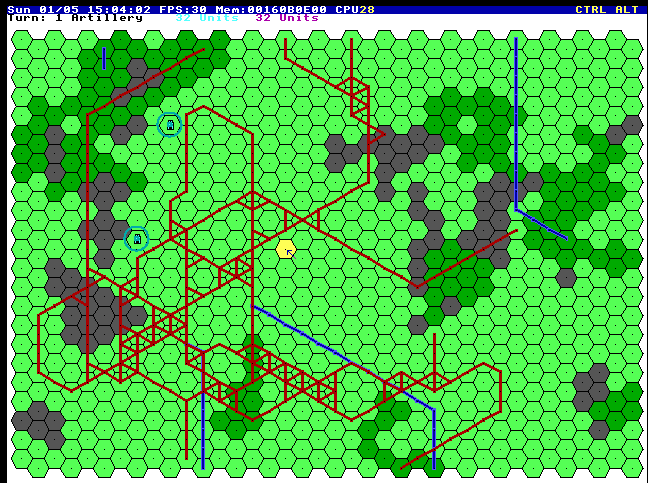
\includegraphics[width=0.6\linewidth]{images/to_the_front.png}
			\caption{To The Front. Own work.}
			\label{fig:to_the_front}
		\end{figure}
	\end{frame}

	\begin{frame}
		\frametitle{Span}
		Bridge building game
		\begin{figure}
			\centering
			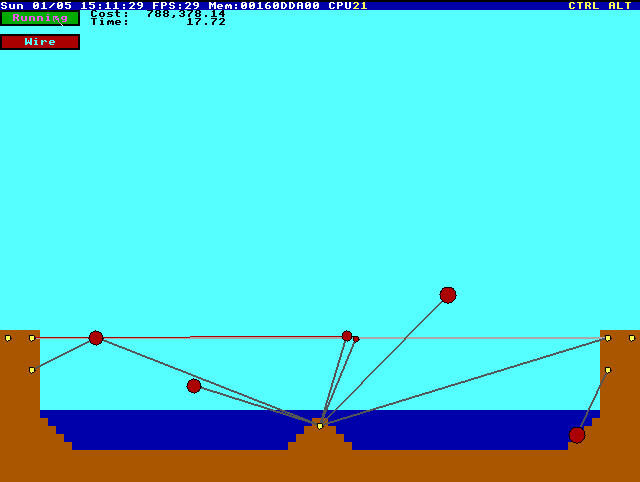
\includegraphics[width=0.6\linewidth]{images/span.png}
			\caption{Span. Own work.}
			\label{fig:span}
		\end{figure}
	\end{frame}

	\begin{frame}
		\frametitle{Tree Checkers}
		Abstract game based on Checkers
		\begin{figure}
			\centering
			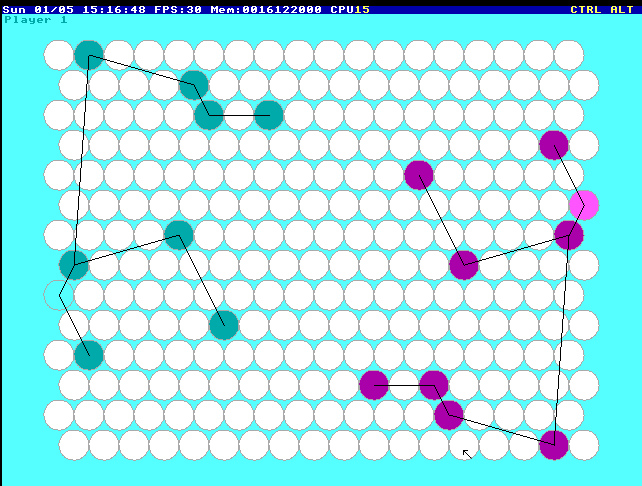
\includegraphics[width=0.6\linewidth]{images/tree_checkers.png}
			\caption{Tree Checkers. Own work.}
			\label{fig:tree_checkers}
		\end{figure}
	\end{frame}

	\begin{frame}
		\frametitle{Digits}
		Game for training short term memory
		\begin{figure}
			\centering
			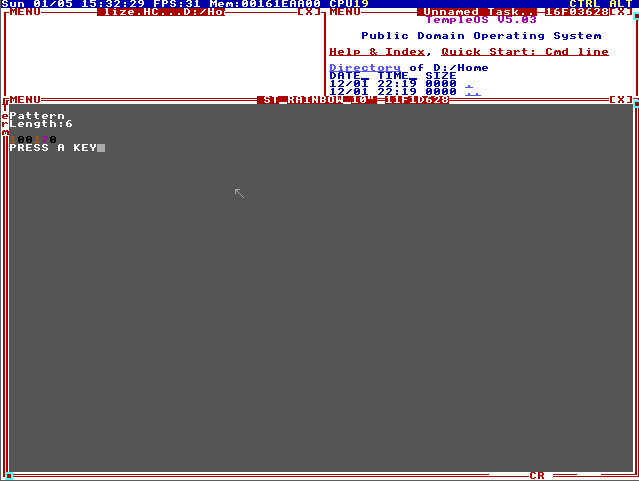
\includegraphics[width=0.6\linewidth]{images/digits.png}
			\caption{Digits. Own work.}
			\label{fig:digits}
		\end{figure}
	\end{frame}

	\subsection{Code Scraps}
	\begin{frame}
		\frametitle{Code Scraps}
		\begin{figure}
			\centering
			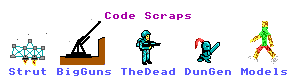
\includegraphics[width=0.5\linewidth]{images/code_scraps.png}
			\caption{Code Scraps. Own work.}
			\label{fig:code_scraps}
		\end{figure}
	\end{frame}

	\begin{frame}
		\frametitle{Strut}
		StarWars game - spaceship constructing strategy
		\begin{figure}
			\centering
			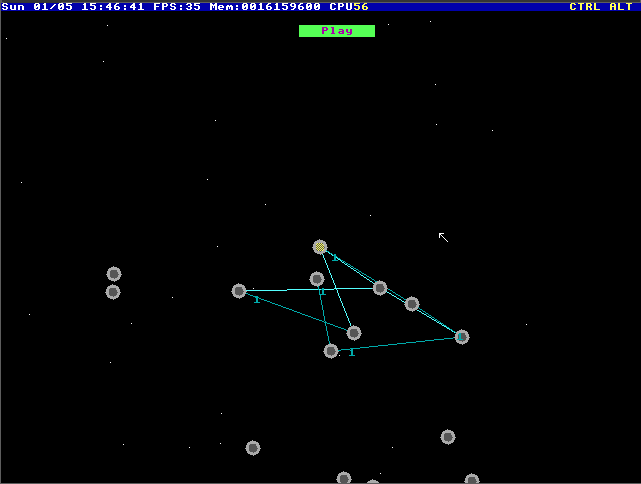
\includegraphics[width=0.6\linewidth]{images/strut.png}
			\caption{Strut. Own work.}
			\label{fig:strut}
		\end{figure}
	\end{frame}

	\begin{frame}
		\frametitle{Big Guns}
		Destroy land with a cannon game
		\begin{figure}
			\centering
			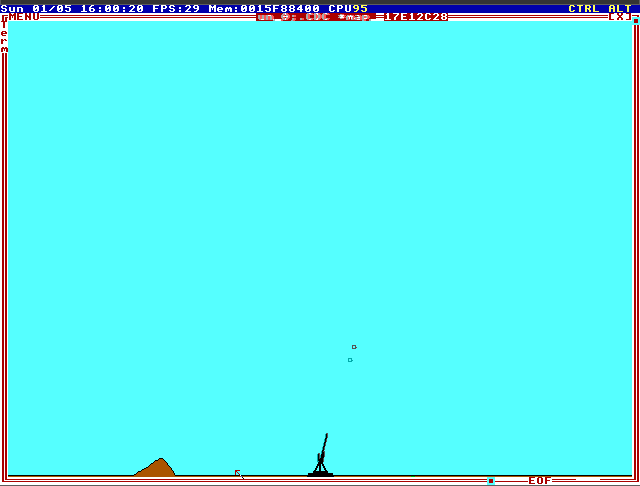
\includegraphics[width=0.6\linewidth]{images/big_guns.png}
			\caption{Big Guns. Own work.}
			\label{fig:big_guns}
		\end{figure}
	\end{frame}

	\begin{frame}
		\frametitle{The Dead}
		Shooter protecting themselves from zombies game
		\begin{figure}
			\centering
			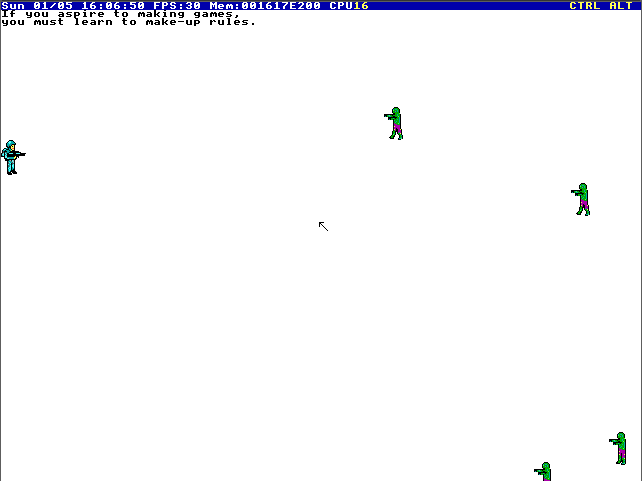
\includegraphics[width=0.6\linewidth]{images/the_dead.png}
			\caption{The Dead. Own work.}
			\label{fig:the_dead}
		\end{figure}
	\end{frame}

	\begin{frame}
		\frametitle{DunGen}
		Kill the enemies game, where the player's vision is limited
		\begin{figure}
			\centering
			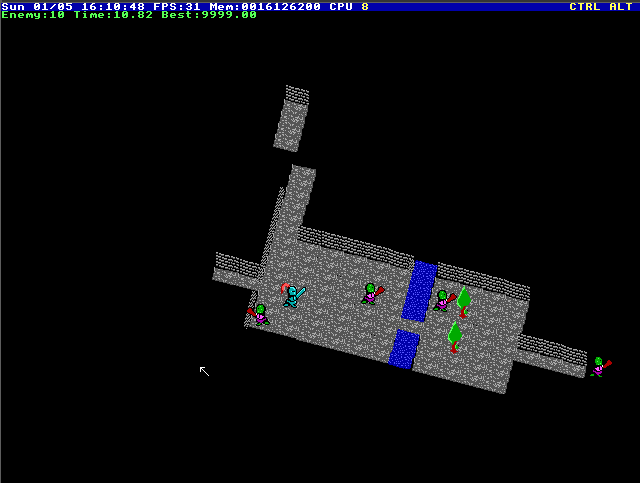
\includegraphics[width=0.6\linewidth]{images/dungen.png}
			\caption{DunGen. Own work.}
			\label{fig:dungen}
		\end{figure}
	\end{frame}

	\begin{frame}
		\frametitle{Models}
		Allows creating models of people and balls
		\begin{figure}
			\centering
			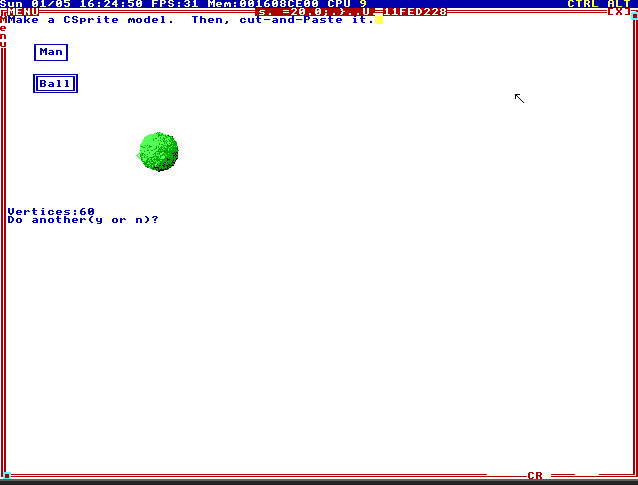
\includegraphics[width=0.6\linewidth]{images/models.png}
			\caption{Models. Own work.}
			\label{fig:models}
		\end{figure}
	\end{frame}

	\subsection{Nongames}
	\begin{frame}
		\frametitle{Nongames}
		\begin{figure}
			\centering
			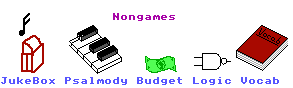
\includegraphics[width=0.5\linewidth]{images/nongames.png}
			\caption{Nongames. Own work.}
			\label{fig:nongames}
		\end{figure}
	\end{frame}

	\begin{frame}
		\frametitle{Jukebox}
		Jukebox with 3 songs
		\begin{figure}
			\centering
			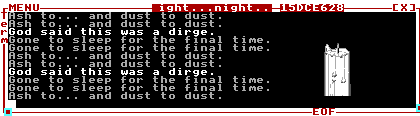
\includegraphics[width=0.6\linewidth]{images/jukebox.png}
			\caption{Jukebox. Own work.}
			\label{fig:jukebox}
		\end{figure}
	\end{frame}

	\begin{frame}
		\frametitle{Psalmody}
		Simple piano program
		\begin{figure}
			\centering
			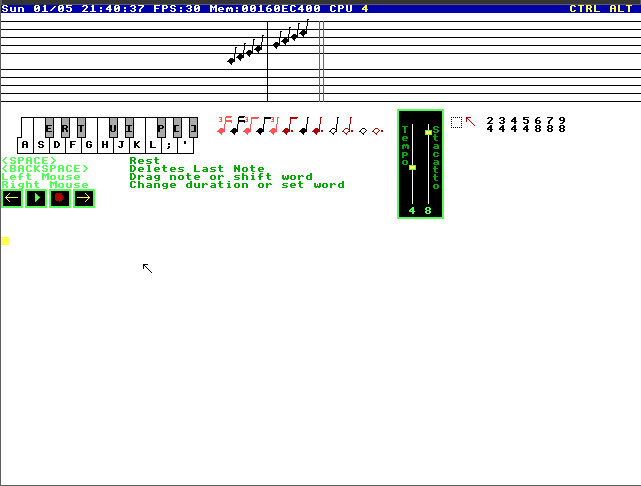
\includegraphics[width=0.6\linewidth]{images/psalmody.png}
			\caption{Psalmody. Own work.}
			\label{fig:psalmody}
		\end{figure}
	\end{frame}

	\begin{frame}
		\frametitle{Logic}
		Logic gates visualization tool
		\begin{figure}
			\centering
			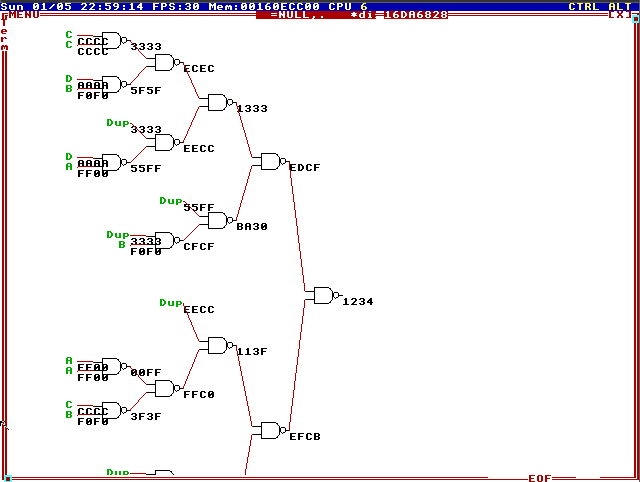
\includegraphics[width=0.6\linewidth]{images/logic.png}
			\caption{Logic. Own work.}
			\label{fig:logic}
		\end{figure}
	\end{frame}

	\begin{frame}
		\frametitle{Vocab}
		Program to train vocabulary
		\begin{figure}
			\centering
			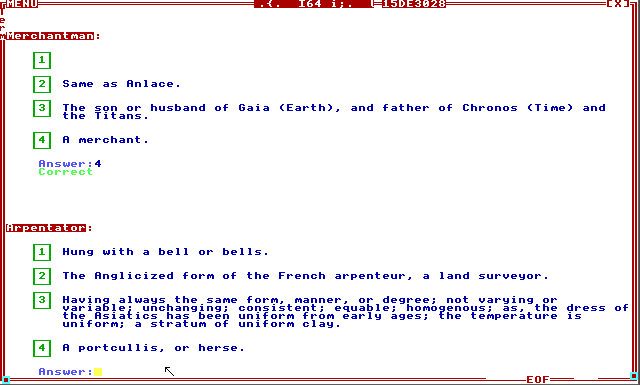
\includegraphics[width=0.6\linewidth]{images/vocab.png}
			\caption{Vocab. Own work.}
			\label{fig:vocab}
		\end{figure}
	\end{frame}

	\section{HolyC}
	\subsection{HolyC introduction}
	\begin{frame}
		\frametitle{HolyC}
		\begin{columns}
			\begin{column}{0.6\textwidth}
				\begin{itemize}
					\item Stands between C and C++

					\item Community compilers for MacOS and Linux

					\item Uses Just In Time compiling

					\item No main() function

					\item Specific traits shown on next slides
				\end{itemize}
			\end{column}
			\begin{column}{0.4\textwidth}
				\begin{figure}
					\centering
					\includesvg[width=0.8\textwidth]{images/HolyC_Logo.svg}
					\caption{HolyC logo}
					\label{fig:HolyC_logo}
				\end{figure}
				Image by \cite{1ctinus_english_2020}.
			\end{column}
		\end{columns}
	\end{frame}

	\subsection{Specific traits of HolyC}
	\begin{frame}
		\frametitle{Holy C - Base types}
		\begin{itemize}
			\item F64 - 64-bit floating point type

			\item U64 - Unsigned 64-bit Integer type

			\item I64 - Signed 64-bit Integer type

			\item U32 - Unsigned 32-bit Integer type

			\item I32 - Signed 32-bit Integer type
		\end{itemize}
	\end{frame}

	\begin{frame}
		\frametitle{Holy C - Base types}
		\begin{itemize}
			\item U16 - Unsigned 16-bit Integer type

			\item I16 - Unsigned 16-bit Integer type

			\item U8 - Unsigned 8-bit Integer type

			\item I8 - Signed 8-bit Integer type

			\item Bool - Signed 8-bit Integer type

			\item U0 - void type
		\end{itemize}
	\end{frame}

	\begin{frame}[fragile]
		\frametitle{Holy C - Functions}
		\begin{itemize}
			\item Invoked without arguments

			\item Default arguments allowed at any point in the definition

			\item The , sign allows logical order

			\item ... for variable argument counts

			\item for loops don't require \{ and \}

			\item No Main() function
		\end{itemize}
	\end{frame}

	\begin{frame}[fragile]
		\frametitle{Holy C - Switch case}
		\begin{itemize}
			\item More efficient than if statements

			\item Implemented with a jump table

			\item Can be nested as sub switch too
		\end{itemize}
	\end{frame}

	\begin{frame}[fragile]
		\frametitle{Holy C - \#exe\{\}}
		This feature allows programs to insert text into the compiled stream of code.
	\end{frame}

	\subsection{Code Examples}
	{
	\begin{frame}[fragile]
		\frametitle{Holy C - Hello World}
		\begin{lstlisting}[language=HolyC]
    U0 Hello(){
    "Hello World\n";  
    }
    Hello;
\end{lstlisting}

		Code by \cite{barretone_barrettottetempleos-and-holyc_2018}.
	\end{frame}

	\begin{frame}[fragile]
		\frametitle{Holy C - Switch}
		\begin{lstlisting}[language=HolyC]
    I64 i;
      for (i=0;i<20;i++) 
        switch (i) {
          case: "Zero\n";   break; 
          case: "One\n";    break; 
          case: "Two\n";    break;
          case: "Three\n";  break;
          case 10: "Ten\n"; break;
          case: "Eleven\n"; break; 
      }
\end{lstlisting}

		Code by \cite{zealos_zeal-operating-systemzealos_2025}.
	\end{frame}

	\begin{frame}[fragile]
		\frametitle{Holy C - \#exe\{\}}
		\begin{lstlisting}[language=HolyC]
    #exe {
    if (!kernel_cfg->mount_ide_auto_hd_let)
      kernel_cfg->mount_ide_auto_hd_let='C';
    if (!kernel_cfg->mount_ide_auto_cd_let)
      kernel_cfg->mount_ide_auto_cd_let='T';
    StreamPrint("blkdev.first_hd_drv_let=%d;",
          kernel_cfg->mount_ide_auto_hd_let);
    StreamPrint("blkdev.first_dvd_drv_let=%d;",
          kernel_cfg->mount_ide_auto_cd_let);
  }
\end{lstlisting}

		Code by \cite{davis_terry_2017}.
	\end{frame}

	\begin{frame}
		\frametitle{Holy C - Useful websites}
		\begin{itemize}
			\item Website with documentation:

				\url{https://holyc-lang.com/}

			\item Compiler for Linux and MacOS:

				\url{https://github.com/Jamesbarford/holyc-lang}
		\end{itemize}
	\end{frame}

	\section{Forks}
	\subsection{ZealOS}
	\begin{frame}
		\frametitle{ZealOS}
		\begin{itemize}
			\item Modernized version

			\item 32-bit colors

			\item 60 FPS

			\item Scalable resolution

			\item Allows networking using Ethernet
		\end{itemize}
		\url{https://github.com/Zeal-Operating-System/ZealOS}
	\end{frame}

	\begin{frame}{ZealOS}
		\begin{columns}
			\begin{column}{0.7\textwidth}
				\begin{figure}[h]
					\centering
					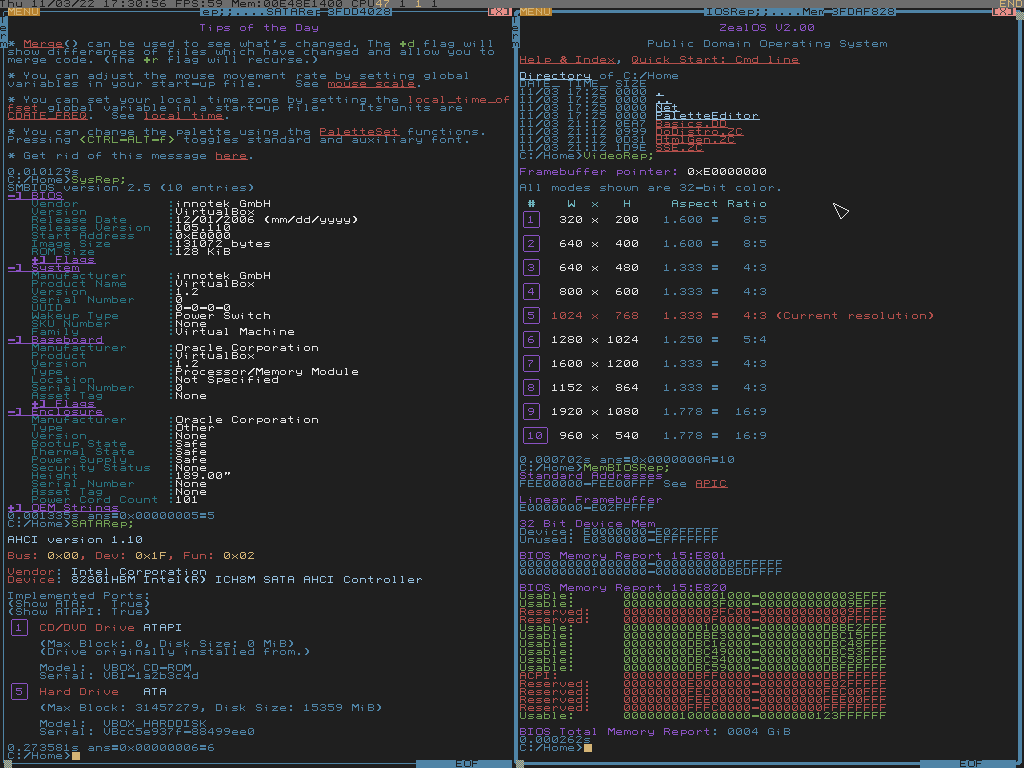
\includegraphics[width=0.8\linewidth]{images/zeal_os.png}
					\caption{ZealOS}
					\label{fig:ZealOS}
				\end{figure}
			\end{column}
			\begin{column}{0.2\textwidth}
				\begin{figure}
					\centering
					
\includegraphics[width=1.0\linewidth]{images/zealos_logo.png}
					\caption{ZealOS logo}
					\label{fig:zealos_logo}
				\end{figure}
			\end{column}
		\end{columns}
		\centering
		Both images by \cite{zealos_zeal-operating-systemzealos_2025}.
	\end{frame}

	\subsection{ZenithOS}
	\begin{frame}
		\frametitle{ZenithOS}
		\begin{itemize}
			\item 60 FPS

			\item VBE graphics with variable resolutions

			\item HolyC replaced with CosmiC.

			\item Reformated code with renamed functions

			\item 32-bit colors
		\end{itemize}
		\url{https://github.com/PasqualeLivecchi/ZenithOS}
	\end{frame}

	\begin{frame}{ZenithOS}
		\begin{figure}[h]
			\centering
			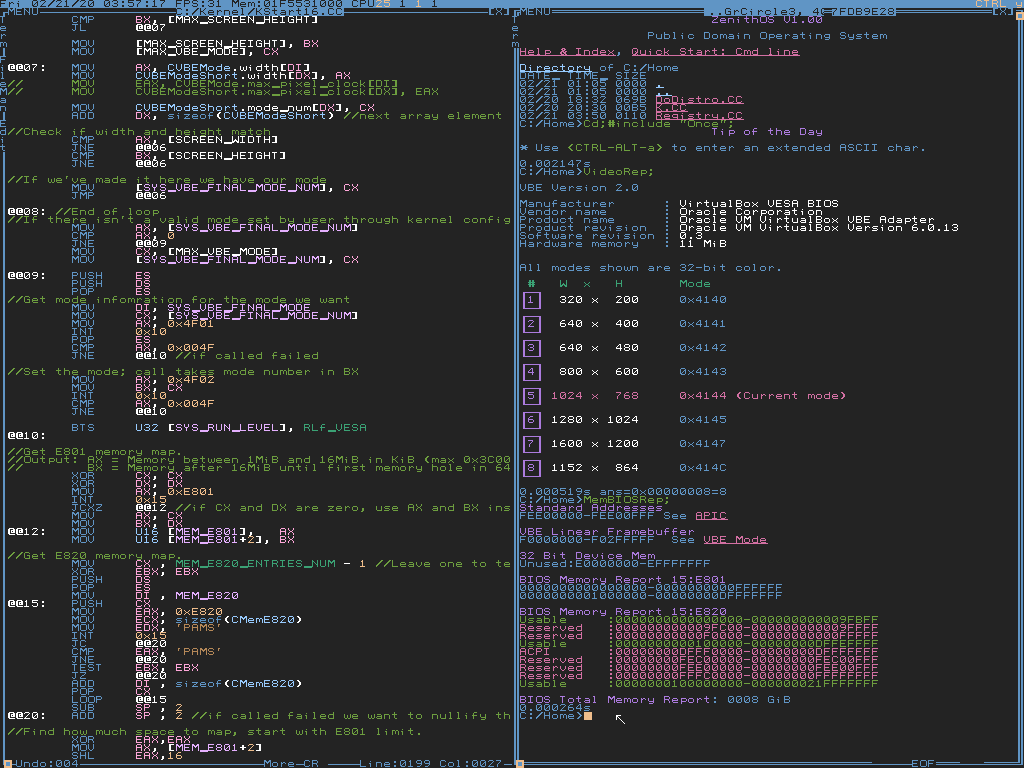
\includegraphics[width=0.6\linewidth]{images/zenith_os.png}
			\caption{ZenithOS}
			\label{fig:ZenithOS}
		\end{figure}
		Image by \cite{livecchi_pasqualelivecchizenithos_2024}
	\end{frame}

	\subsection{TinkerOS}
	\begin{frame}
		\frametitle{TinkerOS}
		\begin{itemize}
			\item Improved installer

			\item More apps (eg. AfterEgypt)

			\item Screenshots

			\item API extensions
		\end{itemize}
		\url{https://tinkeros.github.io/WbGit/}
	\end{frame}

	\begin{frame}{TinkerOS}
		\begin{figure}[h]
			\centering
			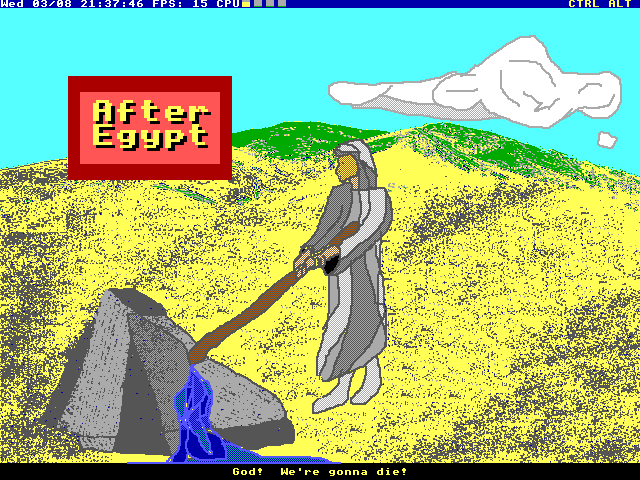
\includegraphics[width=0.6\linewidth]{images/after_egypt.png}
			\caption{AfterEgypt}
			\label{fig:AfterEgypt}
		\end{figure}
		Image by \cite{tinkeros_tinkeros_2024}.
	\end{frame}

	\subsection{Shrine}
	\begin{frame}
		\frametitle{Shrine}
		\begin{itemize}
			\item Package downloader

			\item Lambda Shell (more UNIX-like)

			\item TCP/IP internet access

			\item Origin from the Czech Republic
		\end{itemize}

		\vspace{1em}
		\begin{quote}
			Shrine is a TempleOS distribution full of sin. \flushright - Minexew
		\end{quote}
		\url{https://github.com/minexew/Shrine}
	\end{frame}

	\begin{frame}{Shrine}
		\begin{figure}[h]
			\centering
			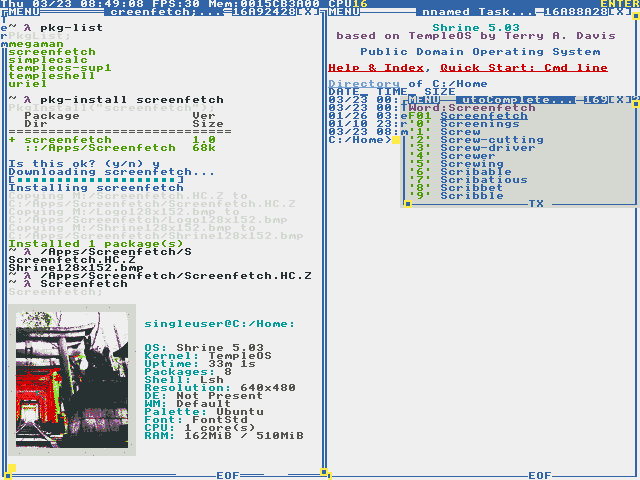
\includegraphics[width=0.6\linewidth]{images/shrine.png}
			\caption{Shrine}
			\label{fig:Shrine}
		\end{figure}
		Image by \cite{minexew_minexewshrine_2020}.
	\end{frame}

	\begin{frame}[allowframebreaks]
		\frametitle{References}
		\nocite{*}
		\printbibliography
	\end{frame}
\end{document}